\chapter{Previous work} \label{sec:previous_work}
\section{Food localization}

%% Color and edge segmentation
%% 11.1

A way to localize food is based on edge detection and colour segmentation.

In \cite{Thendral2014a}, the authors describes and compare these two methods to localise an orange in a picture. It applied these methods on a small dataset of 20 orange images (only one orange per image), with different lighting conditions and backgrounds (pictures are taken from the Internet).
In more details, the edge-based segmentation apply the canny-edge segmentation, then apply non-maximum suppression to eliminate noises. Then, each pixels are classified.
The colour-based segmentation normalised the lightning condition with a Gaussian low-pass filter, convert the RGB image into a $L * a * b$
\begin{enumerate}
    \item Gaussian low pass filter to normalize the lightning condition
    \item convert the image from RGB representation to $L * a * b$
    \item use the $a$ channel to classify each pixel as \enquote{fruit} or \enquote{non-fruit}
    \item remove small object
    \item fill the binary image regions and holes
\end{enumerate}
For orange detection, the colour segmentation has an higher accuracy. Yet, it is very hard to generalise this method.

%% Circle
%% 2.2 (partial) + 6.3 + \cite{Dehais2015} ?

An other method for food detection relies on circle detection. Indeed, food items are often served in a round shape container such as a bowl, pan or plate.

In \cite{Wazumi2011}, the authors describe their use of the Hough transformation to detect circle (they constitutes the food region).

%% CNN
%% DCNN: * ? + 9.1 (in food intake)

A more recent development is the used of convolutional neural network.

In \cite{Shimoda2015}, the authors presents their segmentation process based on a pre-trained deep CNN.

The proposed pipeline is composed of 6 main steps:
\begin{enumerate}
    \item detect all the possible bounding box (maximum 2000 per image) using selective search
    \item cluster the bounding box, using the ration of intersection over union (IOU, also call overlap ratio) to obtain 20 at most.
    \item a Deep CNN for all the selected bounding box to get a saliency map. The DCNN is modelled on AlexNet CNN, was pre-trained on the Salient Object Subitizing (14 000 everyday pictures) dataset and fine-tuned on UEC FOOD 100.
    \item use the GrabCut algorithm to extract the foreground region from the food area. 
    \item In case of overlapped bounding box, the authors proposed to apply the non-maximum suppression (NMS) algorithm.
\end{enumerate}

The authors apply this process on the UEC-FOOD 100 dataset and PASCAL VOC 2007. The latter is used for object detection and recognition of 20 common classes (train, tv, cat, human ...)). These two datasets use bounding box to spot items. A segmentation is correct if the overlap ratio exceeds 50\% between the predicted and the ground truth bounding box.

For UEC-FOOD 100, the authors obtain 49.9 \% mean average accuracy and 58.7 \% for PASCAL VOC 2007.

\section{Food recognition}

Food recognition

Using SVM:

Local using BOW: 3.3
global feature:
Colour and texture description: 
Spatial pyramid:

Mix of several features:

%% DCNN
%% 2.3

More recently, people have started to heavily use Convolutional Neural Networks \textit{CNN} with great results.

In \cite{Kawano2014}, the authors use a pre-trained Deep CNN \textit{DCNN} for feature extraction. The DCNN, called OverFeat, \footnote{Can be found \url{http://cilvr.nyu.edu/doku.php?id=code:start}} was trained on ImageNet and is composed of 19 layers. The authors add more conventional image features to obtain feature vectors composed of: 
\begin{enumerate}
    \item a variant of the Histogram of Oriented Gradients \textit{HOG} called \enquote{RootHog} that is an element-wise square root of the L1 normalized HOG
    \item mean and variance values of each channel of the RGB representation value of pixels from each of 2*2  block
    \item the last two layers of the DCNN
\end{enumerate}
The three descriptors are then encoded in a fisher vector. Using SVM, the authors obtain 72\% of accuracy for UEC-FOOD 100.

\cite{Yanai2015} use a fine-tuned DCNN, pre-trained on 2000 classes (including 1000 food classes) from ImageNet. The authors obtain 78 \% accuracy on UEC-FOOD 100 and 68 \% for UEC-FOOD 256. This dataset, presented in \cite{Kawano2015}, is an extension of 256 classes of UEC-FOOD 100 using a so-called \enquote{foodness classifier} and transfer learning on images coming from crowdsourcing.
In \cite{Bolanos2016}, the authors use a pre-trained DCNN on UEC-FOOD 256.

\section{Food intake estimation}

%% Food Log

FoodLog \footnote{\url{http://www.foodlog.jp}} is a website that enables the user to upload pictures of its daily meals to be archived and processed. The goal of this application is to assist the user to keep notes of their meals and balance the nutritional values coming from different kinds of food.

In \cite{Kitamura2008}, the images containing food items are identified by exploiting features related to the HSV and RGB colour domains, as well as the shape of the plate. A SVM classifier is trained to detect food images. More specifically, the images are divided in 300 blocks and each block is classified as \enquote{non-food} (discarded block) or one of the nutritional categories described in the \enquote{MyPyramid} model \footnote{\url{http://www.mypyramid.gov}}.

MyPyramid \cite{MyPyramid} was designed by the United State Department of Agriculture \textit{USDA} in 2005 and was replaced in 2011 by \enquote{MyPlate} \footnote{\url{http://www.choosemyplate.gov}} \cite{MyPlate}. This dietary model is composed of 5 kinds of food: grains, vegetable, meals and beans, milk and fruit. For each group, a recommended intake per day is associated, Fig. \ref{fig:my_pyramid}. Quantity is categorized by \enquote{servings} \textit{SV}, making it simpler to compute and keep log.

\begin{figure}
    \centering
    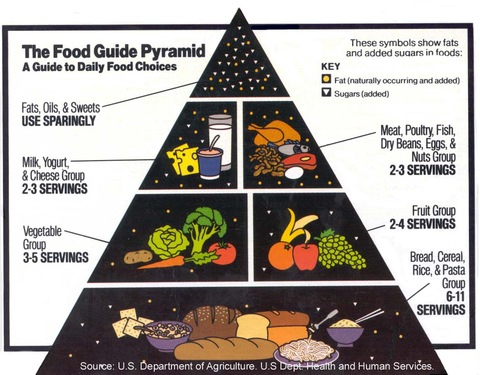
\includegraphics[scale=0.8]{img/my_pyramid.jpg}
    \caption{USDA MyPyramid original logo}
    \label{fig:my_pyramid}
\end{figure}

In \cite{Aizawa2013} the Support Vector Machine is replaced by a Bayesian Framework \textit{BF}.
The BF is based on the Gaussian Naive Bayesian (suppose independence between every pair of features and the distribution of each feature is assumed to be Gaussian). The BF takes into account the estimation using colour moments and Bag-Of-Feature of SIFT, the prior distribution and the mealtime category (breakfast, lunch and dinner).

In \cite{Kagaya2014}, the authors use a Convolutional Neural Network \textins{CNN} to detect and classify food from a small subset of image loaded in the FoodLog system. Compared to the other conventional methods (use of a feature descriptor such as Bag-of-Words with a classifier, e.g. SVM) described previously, the CNN showed a significantly higher accuracy.

%% Others

An other method to estimate the food intake is to evaluate the food volume.

In \cite{Chen2012}, the authors presents a method that use the depth information of the picture. Once the food has been classified, the area of the food container (bowl, plate) and the depth value of the contained food is computed to obtain the food volume.
Yet, this technique is still limited as it can only be used for non-transparent food, i.e it can't detect some food item such as water or cooked rice, and force the user to have a depth camera (such as Kinect).

In \cite{Almaghrabi2012a}, the authors presents a novel food recognition system that is able to estimate of the nutrition intake. Moreover, they develop a mobile application to easily take pictures and keep track of the user's diet.
To measure the food intake, authors compare before and after eating pictures and use the thumb as the calibration system (it supposes a one-time calibration to know the size of the thumb of the user).
The process to show the intake is:
\begin{enumerate}
    \item the user takes food pictures
    \item get the contour of each picture
    \item recognition of the food using colour, shape and size features with SVM.
    \item volume calculation, that is computed in two steps:
    \begin{enumerate}
        \item user takes a picture from above. Then, the food shape is divided into known shape (rectangle, circle, triangle ...) to compute the area.
        \item user takes a second picture from the side. This is used to compute the height of the food and calculate the overall volume.
    \end{enumerate}
    The system assumes that the plate is white and round.
    \item use a nutrition database to obtain the average calories
\end{enumerate}
If the user has not eaten everything, the entire must be repeated.
The drawbacks of this method is the user have to take several pictures, with one's thumb each time and it has been tested with a limited set of simple food types.

%
% Zhu
%

In \cite{Zhu2010}, the authors develop a mobile application to keep food records of a user that is taking pictures of one's meal. Their method can detect multiple food items in one picture. They use a colour marker (color chequerboard) as an illumination and size indicator.
As in \cite{Almaghrabi2012a}, images obtained before and after foods are eaten are used to estimate the amount of food consumed.

When the user upload a picture, it is segmented, then classified by a back-end server. The estimation (labelled image with food type and volume) are sent back to the user for confirmation.

For segmentation, the authors use connected component analysis, active contours, and normalized cuts. Then, colour and texture features are extracted to feed a SVM classifier. The authors use:
\begin{itemize}
    \item Gabor filters. Gabor filters describe properties related to the local power spectrum of a signal and have been used for texture analysis
    \item 2-D colour histograms of the a* and b* channels of the CIELaB representation. Values are corrected using the colour marker
\end{itemize}
For the volume estimation, the authors use a 3-D volume reconstruction process. The food area is partitioned and assigned to \enquote{geometric classes}, each with their own sets of parameters.

They evaluate their segmentation and classification methods on a very small dataset composed of 63 images and 19 classes. The authors obtain an average accuracy of 89 \%.

In \cite{Zhu2015}, their method is named \enquote{multiple hypotheses segmentation and classification} \textit{MHSC}. It is an iterative algorithm composed of a segmentation, description (extraction of features) and classification steps.

For segmentation, the authors first detect salient region, using Canny edge and colour distribution to reject background. Then, they apply a multi-scale segmentation using normalized cut. Small segmented regions are discarded.

On the selected region, the authors used a mixed of global descriptors (first and second moment of each channel for RGB, YCbCr, L*a*b*, and HSV colour spaces, first and second moment of the entropy in RGB, predominant colour descriptor, entropy and two first moments of the Gradient Orientation Spatial-Dependence Matrix, entropy categorization and fractal dimension estimation and estimation of the fractal dimension of the response of different Gabor filter) with local feature (multi Bag-Of-Words using SIFT for RGB, SURF for RGB, SIFT for each channel of the RGB representation and steerable filters).

Each of the 12 descriptor, global and local, is classified independently and assigned a confidence score. A late fusion function (either maximum confidence score or majority vote) is used  to decide the final class. For classification, the authors use K-NN and SVM.

If the total score is inferior to a certain threshold, the overall process is repeated. The confidence score of the previous step is used to improve the segmentation.

Applied on a dataset composed of 83 labels (79 food classes plus \enquote{utensils}, \enquote{glasses}, \enquote{plates}, and \enquote{plastic cups} classes), each class having at least 30 images, they obtain a top-8 accuracy of 75 \%, using K-NN with the maximum confidence score.

%% Food Cam
%% 6.3

In \cite{Matsuda2012a}, the authors propose a food recognition system named \textbf{FoodCam} to identify food items of a picture. The presented process is used on a mobile application, the user taking a picture that is transferred to a sever, processed and results are displayed.

The first step is to detect potential region with multiple object detection algorithms. Then, for these regions, several feeatures are extracted and used to feed SVM with Multiple Kernel Learning \textit{MKL} method. To detect candidate regions, the authors use:
\begin{itemize}
    \item Felzenszwalb’s deformable part model (DPM), based on Histogram of Oriented Gradients (HOG).
    \item a circle detector: the image is converted to a gray-scale, contour are extracted using the Canny Edge Detector and circles detected by the Hough Transform
    \item JSEG region segmentation: segment region based on colour. It only keeps circular regions.
    \item whole image, for picture with one large dish
\end{itemize}
Then, it aggregates all the candidate regions to get the bounding box of each food item.

For each region, it extracts multiple common features:
\begin{itemize}
    \item Bag of Feature of SIFT and C-SIFT (sift with colour invariant characteristics)
    \item Spatial pyramid representation: object regions are divided by hierarchical grids. In this paper, the three level pyramid is used: $1 \times 1$, $2 \times 2$, $3 \times 3$. For each grid, a BoF vector is extracted
    \item Histogram of Oriented Gradient (HOG)
    \item Gabor texture
\end{itemize}

After extraction of the feature vectors from each candidate region, a linear SVM trained by MKL is used ($\chi^2$ kernel).

For evaluation, the authors build a new dataset composed of 100 categories of traditional Japanese dishes with their associated bounding boxes for a total of 9060 images named \textbf{UEC-FOOD 100}. For multiple food item images, they obtain 55.8 \% classification rate and 68.9 \% for single food item pictures.

In \cite{Kawano2014a}, the authors develop a mobile real-time food recognition system for calorie and nutrition estimation. Contrary to the previous paper, all the calculation are realised on the user smartphone. The recognition takes less than 1 second thanks to the multi-core architecture of modern smartphones.
The user takes a picture and draws bounding boxes around food items. Then, the system refine the segmentation based on the users' rough demarcation using Grabcut, an iterative method using graph cuts to extract foreground.
For each item, it extracts image features and classify the image among the one hundred food classes using a linear SVM. Then, the top five food candidates are shown and the user can select one of the proposition.
This recognition is updated every one second, the direction arrow as presented in figure  \ref{fig:food_cam} being displayed to help the user improve the result by changing the camera position and direction. To estimate the most suitable direction, the authors use the Efficient Sub-window Search method, a recent and powerful window search algorithm used in object detection.
The mobile application keep records of all the pictures and their approved classification and labeled with the volume estimation. Food intake is estimated thanks to a slider on the bottom-left of the screen.

\begin{figure}
    \centering
    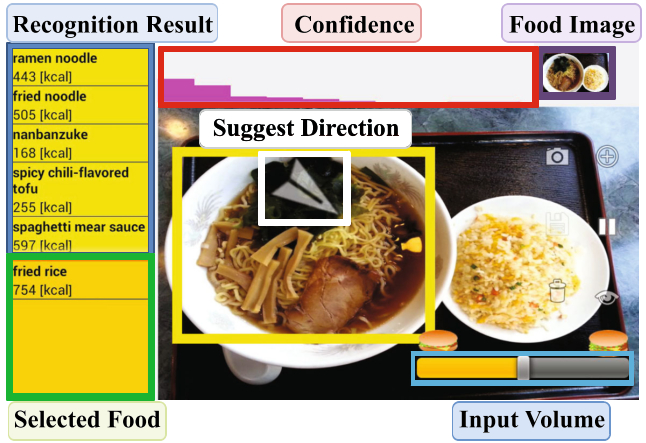
\includegraphics[scale=0.6]{img/foodcam.jpg}
    \caption{Annotated screenshot of the FoodCam application}
    \label{fig:food_cam}
\end{figure}

Two different descriptors are used:
\begin{itemize}
    \item bag-of-feature, SURF for detection and description, and colour histogram with the $chi^2$ kernel feature map
    \item HOG and a colour patch descriptor (mean and variance of RGB values on a $2 \times 2$ blocks of pixel) encoded using Fisher Victor, a patch encoding strategy using Gaussian mixture models.
\end{itemize}
The authors evaluate these two methods on UEC-FOOD 100. Taking the top 5 classes, they obtain 79 \% classification accuracy for colour patches and 68 \% for the other.